\documentclass{article}
\usepackage[utf8]{inputenc}
\usepackage{listings}
\usepackage{geometry,tikz,pgfplots,multicol,relsize,enumitem}
\usepackage{mathtools}
\usepackage{graphicx}
\usepackage{amsfonts} 
\usepackage{listings}
\usepackage{amsmath}
\geometry{a4paper,bottom=1.5cm}

\lstdefinestyle{JavaStyle}{
	tabsize=4,
	language=Java,      % choose the language of the code
	basicstyle=\small,     % the size of the fonts that are used for the code
	aboveskip={1.5\baselineskip},
	columns=fixed,
	showstringspaces=false,
	extendedchars=false,
	breaklines=true,
	showtabs=false,
	showspaces=false,
	showstringspaces=false,
	identifierstyle=\ttfamily,
	keywordstyle=\color[rgb]{0,0,1},
	%commentstyle=\color[rgb]{0.026,0.112,0.095},
	commentstyle=\itshape\color{green!40!black},
	stringstyle=\itshape\color{red!90!black},
	numberstyle=\itshape\color{yellow!50!black}
}


\title{Progetto Reti di Calcolatori \\[5em] 
\large Protocollo MQTT Java}
\author{Petreti Andrea\\\small Matricola 272822}
\date{06 Agosto 2016}
\begin{document}


\maketitle
\thispagestyle{empty}

\newpage 

\renewcommand{\contentsname}{Indice}

\tableofcontents

\newpage

\section{Introduzione}
Si vuole implementare un noto protocollo di messaggistica chiamato MQTT (Message Queue Telemetry Transport). MQTT è un protocollo M2M, ovvero machine to machine, viene applicato soprattuto al nuovo settore IoT. In particolare è stato progettato per avere un'impatto basso sia a livello di risorse computazioni richieste, sia a livello di occupaazione di banda; basato sul pattern Publish/Subscribe prevede due componenti:
\begin{itemize}
	\item Message Broker
	\item Client MQTT
\end{itemize}
I client MQTT possono iscriversi ad una certa parola chiave detta "Topic", per poi ricevere successivamente dal Broker solo i messaggi che altri Client hanno inviato sullo stesso Topic. Il Broker, similmente all'archiettura Client-Server, svolge il ruolo di ``Server", e come si può intuire dal nome, si occupa di ricevere e smistare i vari messaggi ai vari destinatari, nonchè di mantenere la lista di Topic al quale ogni Client si è iscritto.

\begin{figure}[htbp]
	\centerline{
		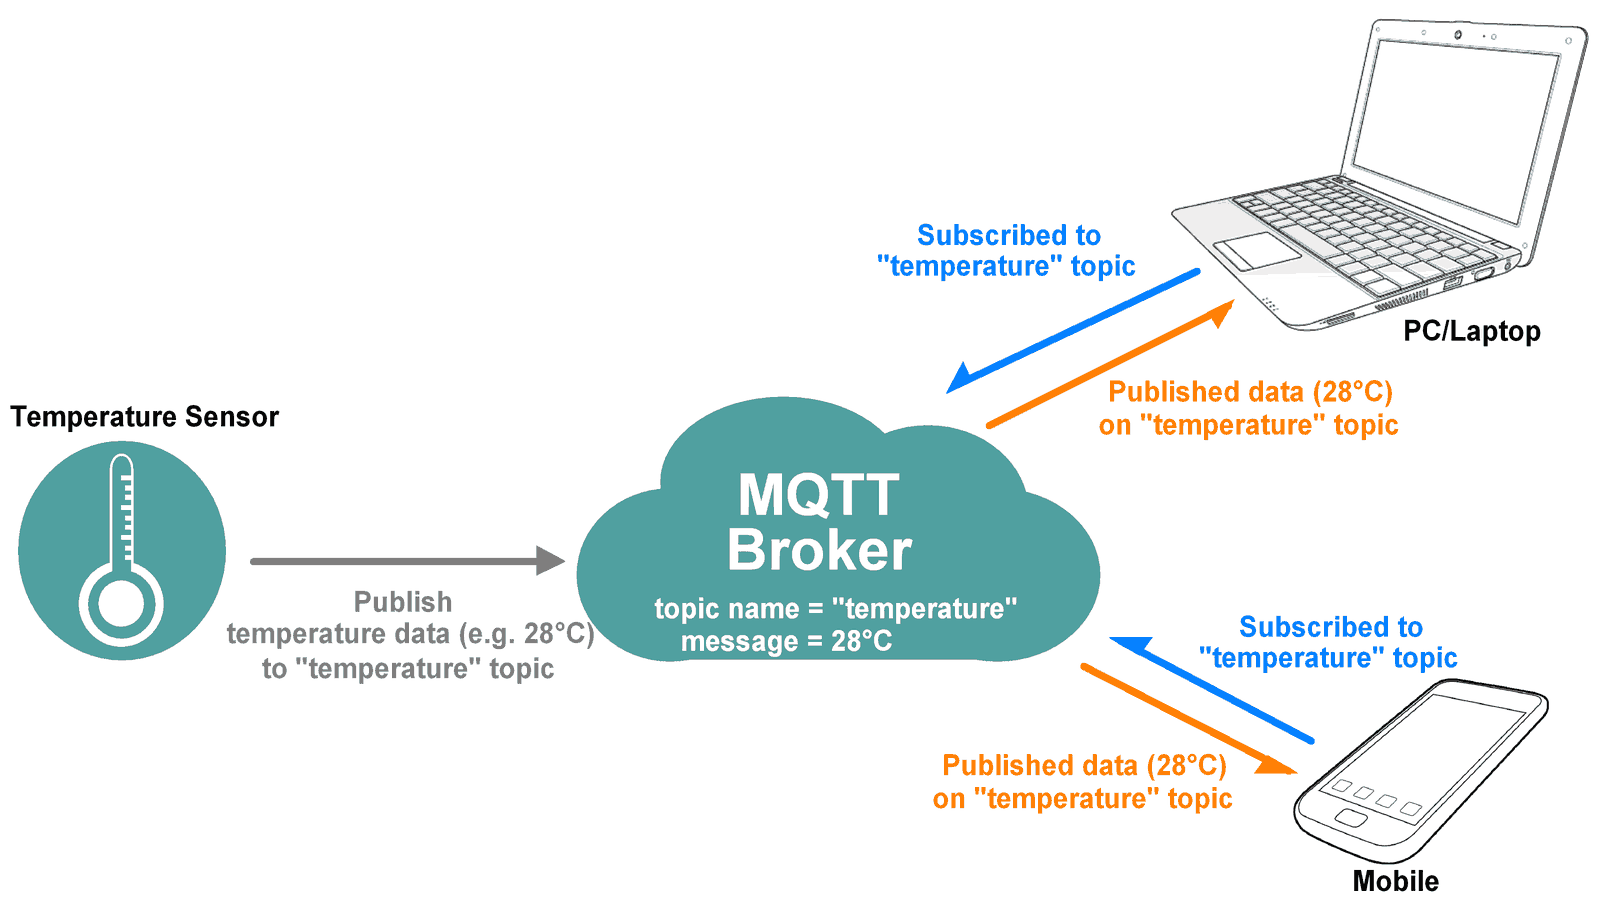
\includegraphics[scale=0.2]{immagini/broker_client_img.png}
	}
\end{figure}

L'immagine mostra un'esempio concreto, abbiamo un sensore di temperatura, che periodicamente invia ``Pubblica" la temperatura registrata, svolgento quindi il ruolo da Cliente che pubblica informazioni al Broker. Mentre il laptop e lo smartphone, si sono iscritti al Topic ``Temperature", e quindi ricevono i dati misurati dal sensore per mezzo del Broker.\\\\
MQTT però ha altre peculiarità, abbiamo detto che si presta bene in situazioni in cui abbiamo banda limitata, questo perchè ogni pacchetto del protocollo MQTT, prevede solo 2 byte di header fisso, inoltre minimizza anche gli scambi di messaggi, mettendo a disposizione tre livelli di servizio, che vengono anche chiamati Qos (Quality of Service).

\begin{figure}[htbp]
	\centerline{
		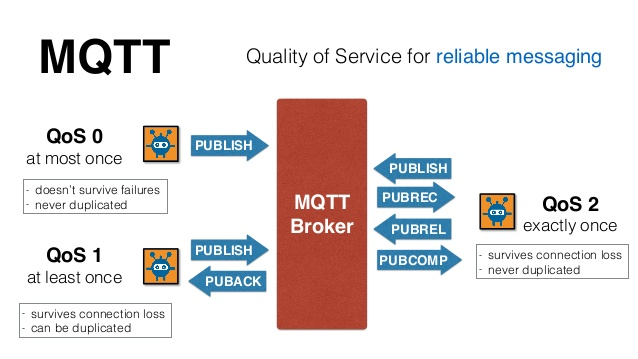
\includegraphics[scale=0.4]{immagini/mqtt_qos.jpg}
	}
\end{figure}

\begin{itemize}
	\item Qos 0 o ``at most once" o ``fire and forget", non da alcuna sicurezza dal punto di vista della mancata consegna o della duplicazione di messaggi, quindi se il messaggio viene perso o duplicato, il Client che ha inviato quel messaggio non può saperlo. Utilizzato nel caso in cui le informazioni non sono necessariamente importanti o nel caso in cui non ci interssa di ricevere messaggi duplicati.
	\item Qos 1 o ``at least once", viene assicurato l'arrivo dei messaggi al Broker, in quanto lui invierà un Ack di conferma, ma possono comunque verificarsi dei casi in cui il messaggio viene duplicato.
	\item Qos 2 o ``exactly once", ci assicura che il messaggio venga consegnato una sola volta e senza duplicazioni, ma l'invio di un message con questo tipo di servizio, aumenta ovviamente l'overhead, in quanto sono richiesti ben 3 Ack successevi da parte del Broker e da parte del Client.
\end{itemize}

MQTT supporta anche un minimo grado di sicurezza, permettendo l'invio nella fase di connessione di un'username e di una password, che poi il Broker dovrà valutare e garantire o meno la connessione, ovviamente in questo caso è necessario utilizzare un livello di transporto come TLS/SSL, oppure criptare e decriptare prima dell'invio e alla ricezione, per evitare che username e password possano essere letti da un'attacco man in the middle.


\section{Composizione Pacchetto MQTT}
Ogni pacchetto MQTT, come detto precedentemente ha un header fisso di 2 byte. Il primo di questi identifica la tipologia del pacchetto, e vari flag.
\begin{itemize}
	\item 4 bit per la tipologia del pacchetto tra cui: Connect, ConnAck, Publish, Subscribe, PubAck, PubRel, PubRec, PubComp, SubAck, Unsubscribe, UnsubAck, Disconnect, PingReq, PingResp.
	\item 1 bit per il flag di duplicazione del messaggio.
	\item 2 bit per la Qos, ovvero al Quality of Service.
	\item 1 bit per il flag Retain, di cui parlero nella sezione dedicata alla pubblicazione di un messaggio.

\end{itemize}Il secondo byte invece contiene la lunghezza della restante parte del pacchetto (payload), che varia a seconda della tipologia.

\section{Funzioni Principali MQTT}

\subsection{Connessione e Disconnesione}
La connessione al Broker avviene tramite l'invio di un pacchetto di connessione (Connect), il quale contiene molte informazioni per la gestione da parte del Broker della sessione e del canale di comunicazione. I principali parametri inviati sono:

\begin{itemize}
	\item Nome Protocollo e Versione Protocollo, ovvero una stringa e un valore numerico per indicare la versione di MQTT 3.1 o 3.1.1.
	\item Flag di connessione di 1 byte, tra cui 1 bit per il flag Username, per indicare se nel payload sarà presente uno username, stessa cosa per il flag Password.\\4 bit per Will Flag, Will Qos e Will retain ed infine un bit per la Clean Session. 
	\item Payload che conterrà un ClientID di massimo 23 caraterri UTF-8, che dovrà rappresentare in maniera univoca il Client.
	\item Il topic del messaggio ``Will", la Qos, e il contenuto del messaggio stesso.
	\item Username e Password, obbligatori a seconda di come sono stati impostati i precendenti Flags.
\end{itemize}
Il Broker quando riceve un richiesta di connessione, deve verificare l'intero pacchetto, controllando la coerenza tra Flags e Payload, nonchè effettuare l'autenticazione se username e password sono stati impostati. Infine il Broker risponde con un pacchetto ``ConnAck", che contiene un codice per indicare lo stato della connessione (Accetata, Autenticazione fallita, ecc..) e un flag che segnala la presenza o meno di una sessione persistente sul Broker per quel Client.\\\\La disconnessione invece avviene in maniera molto semplice, e solo da parte del Client, ovvero solo quest'ultimo, quando vuole disconnetersi invia un pacchetto ``Disconnect" e chiude la connessione. Il Broker invece non può inviare un pacchetto di Disconnect, ma soltanto riceverlo, e alla ricezione, anch'esso chiude la connessione, in tutti gli altri casi quando il broker si disconnette per un qualche errore chiude semplicemente la connessione. Ad esempio una delle politiche MQTT è che quando due client con stesso ClientID tentano di connetersi, il Broker deve disconnetere il meno recente, e lo fa chiudendo la connessione.


\subsection{Sessione}
La Sessione su MQTT, assume un comportamento differente a seconda del valore del flag CleanSession inviato all'atto della connessione. Nello specifico la sessione del Client non è persistente e contiene:
\begin{itemize}
	\item Tutti i messaggi con Qos1 o Qos2 che sono stati inviati al Broker, ma che ancora esso non ha confermato con degli Ack.
	\item Tutti i messaggi con Qos2 che sono stati ricevuti dal Broker, ma che ancora non sono stati completamente confermati, ovvero che non tutti i pacchetti PubRel, PubRec e PubComp sono stati scambiati.
\end{itemize}
La sessione memorizzata dal Broker per ogni Client, invece è persistente se il flag CleanSession è falso, altrimenti la sessione viene eliminata al momento della disconnessione, inoltre contiene più dati rispetto alla sessione del client:
\begin{itemize}
	\item Tutti i Topic a cui il Client è sottoscritto.
	\item Messaggi Qos1 e Qos2 che sono stati inviati al Client, ma ancora non confermati completamente da Ack.
	\item Messaggi Qos1 e Qos2 che sono in attessa di essere inviati al Client.
	\item Messaggi Qos2 che sono stati ricevuti dal Client, ma ancora non complemetamente confermati dallo scambio degli Ack di Qos2.
\end{itemize}
Il vantaggio di avere una sessione persistente, è che quando un client (chiamimolo Pippo) si disconnette la sessione resta salvata sul Broker, e tutti i messaggi che arrivano da altri client verso Pippo (in base ai Topic a cui è iscritto), vengono salvati sulla sua sessione. Quando Pippo si riconnette, il Broker inoltra tutti i messaggi destinati a lui, ma che non ha potuto ricevere in quanto offline. Inoltre Pippo non deve riscriversi ai Topic, poichè il Broker li conosce già dalla sessione. Questo ad esempio è molto utile quando si ha una rete con poca banda, o quando si hanno dispostivi che vogliamo consumino poco, perchè noi ci iscriviamo soltanto una volta ai Topic di nostro interesse, quindi inviamo soltato una volta i pacchetti di iscrizione, e per ridurre i consumi spegniamo e accendiamo il dispositvo ogni tot. di tempo senza preoccuparci di perdere i messaggi destinati ad esso, in quanto è compito del Broker memorizzarli e reinviarli.


\subsection{Pubblicazione}
La pubblicazione di un messaggio verso il Broker, avviene inviado ad esso un pacchetto MQTT (Publish Packet), che contiene:
\begin{itemize}
	\item Un Flag Retain, per indicare se quel messaggio deve essere salvato dal broker in maniera persistente ed inviato ai Client che si connetteranno e sottoiscriveranno successivamente allo stesso topic del messaggio.
	\item QOS, ovvero la qualità del servizio con la quale si vuole pubblicare quel messaggio al Broker. Qos può valore 0, 1 o 2, ed il Broker risponderà in maniera diversa a seconda della Qos. 
	\item Topic, ovvero la parola chiave, che identifica il canale in cui il messaggio verrà pubblicato.
	\item Messaggio, ovvero ciò che si vuole effettivamente pubblicare, come ad esempio un valore di temperatura, un messaggio testutale, ecc...
\end{itemize}
Il Broker dovrà invece:
\begin{itemize}
	\item Controllare quali Client sono sottoscritti allo stesso Topic, ed inviare loro il messaggio ricevuto, utilizzando come Qos il minimo tra la Qos del messaggio ricevuto e la Qos che i sottoscrittori hanno richiesto al momento della sottoscrizione.
	\item Salvare il messaggio in maniera permanente ed inviarlo (pubblicarlo) verso i Client che si iscriveranno anche in futuro al Topic del messaggio, se il Flag di retain è impostato.
	\item Inviare un PUBACK verso il Client che effettua la pubblicazione, se la Qos è uguale ad 1.
	\item Inviare un PUBREC verso il Client che effettua la pubblicazione, attendere che quest'ultimo risponda con un PUBREL, e concludere con l'invio di un PUBCOMP, se la Qos è uguale a 2.
\end{itemize}

\subsection{Sottoscrizione}
La richiesta di sottscrizione da parte del Client, avviene inviado al Broker un pacchetto MQTT, chiamato Subscribe Packet, che contiene:
\begin{itemize}
	\item Il classico header fisso, ma con Qos pari ad 1, poichè la sottscrizione prevede un ACK da parte del Broker.
	\item Topic al quale ci si vuole abbonare.
	\item Qos associata al Topic, per indicare che si vogliono ricevere messaggi dal Broker su quel Topic, con una certa Qos.
\end{itemize}
Il Broker all'arrivo di una richiesta di sottoscrizione dovrà:
\begin{itemize}
	\item Inviare un ACK verso il client, ovvero un paccheto del tipo PUBACK, nel quale deve specificare quale Qos il broker può garantire per il Topic richiesto dal Client.
	\item Inviare al Client stesso, se ci sono, i messaggi retain che il Broker aveva salvato per quel determinato Topic.
\end{itemize}
Inoltre il Client ha la possibilità di rimuovere la sottoscrizione ad un certo Topic, inviato un pacchetto ``Unsubscribe", il quale oltre ad avere un intestazione fissa con Qos 1, perchè anche esso prevede un Ack di ritorno, ovvero il UnsubAck, ha come payload il Topic che si vuole rimuovere.

\subsection{Keep Alive}
MQTT prevede un'meccanismo per stabilire se le due parti, ovvero Broker e Client, sono tra loro effettivamente connessi, utilizzando due tipologie di pacchetti: PingReq e PingResp. Al momento della connessione il Client specifica un certo tempo di keep alive al Broker. Quindi entrambi le parti avviano un timer, che viene azzerato ogni volta che arriva un pacchetto.\\
Quando il timer del Client raggiunge il tempo di keep alive, invia una richiesta di Ping, tramite un pacchetto di PingReq al Broker, il quale dovrà rispondere con pacchetto PingResp, se il Client riceve questa risposta entro il tempo di keep alive, la connessione continua, altrimenti viene interotta in quanto si ritiene che il Broker sia offline.\\
Il Broker, invece, quando il suo timer raggiunge il tempo di keep alive, la connessione con il Client viene automaticamente chiusa.\\

\textbf{N.B.} Ovviamente è importante che entrambi impostino una soglia in eccesso e in difetto per il keep alive, in modo tale da considere anche eventuali ritardi dovuti al traffico sulla rete. Ad esempio il Broker imposterà una soglia in eccesso per attendere leggermente oltre il tempo di keep alive, che il client invii almeno un'messaggio prima di chiudere la connessione. Mentre il cliente imposterà una soglia in difetto, per inviare un pacchetto di PingReq, prima del raggiungimento effetivo del tempo di keep alive.

\subsection{Topic Matching}
Un'altra particolarità di MQTT sono ovviamente i Topic, che non sono semplici parole chiave, ma rappresentano un'insieme di livelli di uno o più topic, ad esempio:
\begin{center}
	``/meteo/urbino/\#" o ``/sensor/+/temperature"
\end{center}

Ogni livello è separato dallo slash in avanti ``/", quindi il matching tra topic avviene in maniera particolare, ovvero verificando che i vari livelli combacino tenendono conto dei caratteri speciali ``\#" e ``+".
\begin{itemize}
	\item \# Viene detto Wildcard a Multi Livello, poichè rappresenta tutti i sotto livelli possibili.
	\item + Viene detto Wildcard a Singolo Livello, poichè rappresenta al massimo un sottolivello.
\end{itemize}
Ad esempio il topic ``/meteo/urbino/dati/temperatura" fa matching con il primo esempio. Stessa cosa per topic ``/sensor/raspberry/temperature" che fa matching con il secondo esempio, mentre ``/sensor/raspberry/dati/temperature", non fa matching con il secondo, in quanto al posto del carattere speciale ``+", sono presenti più di un livello.



\section{Implementazione Java}
Il protocollo MQTT precendemente descritto è stato implementato nel linguaggio Java, sia il Broker che il Client. Lo sviluppo è partito dall'implementazione dei vari pacchetti MQTT in oggetti Java, in particolare ogni classe relativa ad un certo tipo di pacchetto, supporta due tipi di operazione:
\begin{itemize}
	\item Creazione del pacchetto e trasformazione di esso in bytes, pronti per essere inviati tramite socket.
	\item Trasformazione e validazione dei bytes ricevuti da socket in oggetto Java.
\end{itemize}
Ciò ha permesso poi di trattare i pacchetti come semplici oggetti Java e quindi di implementare in maniera più semplice il sistema di gestione code e sessione del Broker e del Client. Inoltre poichè ogni pacchetto ha un header fisso, è stata definita una classe padre che ha il ruolo di effetuare il ``parsing" dei bytes letti da socket. Riporto di seguito il costruttore di tale classe:
\begin{lstlisting}[style=JavaStyle]
public MQTTPacket(byte fixedHeader) throws MQTTParseException {
	mCommand = Type.fromInteger((fixedHeader & 0xF0) >> 4);
	mQos = Qos.fromInteger((fixedHeader & 0x06) >> 1);
	mDup = (fixedHeader & 0x08 >> 3) == 1;
	mRetain = (fixedHeader & 0x01) == 1;
}
\end{lstlisting}
Lo stesso costruttore viene invocato ogni volta che un'pacchetto MQTT viene ricevuto. Qui riport invece l'operazione inversa, ovvero la trasformazione in bytes:
\begin{lstlisting}[style=JavaStyle]
public static byte[] GenerateFixedHeader(MQTTPacket.Type type, int remainLength, boolean dup, int qos, boolean retain) {
	byte[] b = new byte[(remainLength > 127) ? 3 : 2];
	byte dup = ((dup ? 1 : 0) & 0x01) << 3;
	byte qos = (qos & 0x3) << 1;
	byte retain = (retain ? 1 : 0) & 0x1;
	b[0] = (byte) (((type.Value() & 0x0F) << 4) | dup | qos | retain;
	if(remainLength > 127) {
		b[1] = (byte) ((remainLength % 128) | 0x80);
		b[2] = (byte) (remainLength / 128);
	} else
		b[1] = (byte) remainLength;
	
	return b;
}
\end{lstlisting}
Come facilmente intuibili dalla parte di codice, in byte 0, ovvero il primo, viene generato in base alla tipologia del pacchetto MQTT, dalla Qos, dal flag retain e duplicate. Il secondo byte invece contiene la lunghezza rimanente del pacchetto (payload).\\\\
Successivamente è stato implementato ``l'algoritmo" che permette di dividere in blocchi di bytes coerenti, ovvero in Header Fisso e Payload, i bytes provenienti da Socket, in pratica si utilizza il secondo byte del pacchetto MQTT, in quanto contiene la lunghezza del payload. La sezione di codice sottostante, in particolare la parte racchiusa nel do-while, estare proprio questa informazione. Inoltre sottolineo che l'algoritmo è fedele a quello che si trova nella documentazione dello standard MQTT 3.1.1. Una volta estratta la lunghezza del Payload, si leggono gli n successivi bytes i quali verrano trasformati in oggetto Java. 
\begin{lstlisting}[style=JavaStyle]
public synchronized MQTTPacket nextMQTTPacket() throws IOException, MQTTParseException {
	byte fixedHeader = (byte) mBufferedInputStream.read();
	if(fixedHeader != -1) // end of stream reached
	{
		Utils.getType(fixedHeader);
		
		int multiplier = 1;
		int length = 0;
		byte tmp;
		do {
			tmp = (byte) mBufferedInputStream.read();
			length += (tmp & 127) * multiplier;
			multiplier *= 128;
			if(multiplier > 128*128*128)
				throw new MQTTParseException("Malformed Remaining Length", MQTTParseException.Reason.INVALID_MQTT_PACKET);
		} while ((tmp & 128) != 0);
		
		// read all packet with length
		byte[] packet = new byte[length];
		if(mBufferedInputStream.read(packet, 0, packet.length) >= 0) {
			return MQTTPacket.parseBody(fixedHeader, packet);
		}
	}
	return null;
}
\end{lstlisting}
Per testare il corretto invio e ricezione dei messaggi, ho utilizzato WireShark, che mi consentiva di intercettare (sniffing) tutto il traffico di rete e di filtrarlo, in questo modo sono riuscito a verificare l'assenza di pacchetti MQTT malformati.
\begin{center}
	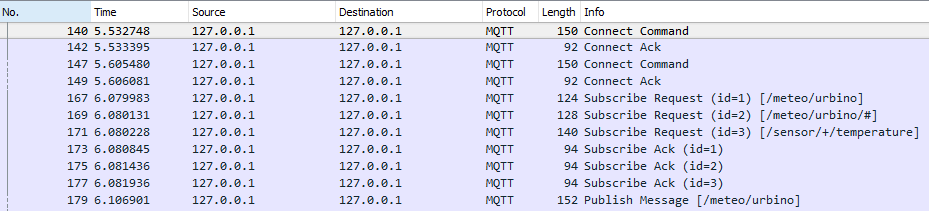
\includegraphics[scale=0.6]{immagini/wireshark1.png}
	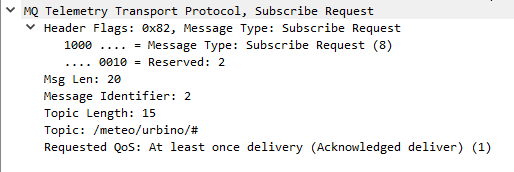
\includegraphics[scale=0.6]{immagini/wireshark2.png}
\end{center}

Definiti quindi tutti i metodi per la lettura di bytes in oggetto Java, definiamo il protocolli di trasport per essi. MQTT utilizza il protocollo TCP, che in Java è facilmente implementabile con delle Socket, ma come detto nelle sezioni precendeti, nonostante MQTT mette a disposizione un sistema di autenticazione, esso è praticamente inutile se non si utilizza un protocollo per cifrare la trasmissione dei dati. In particolare ho deciso di utilizzare TLS v1.2, per migliorare la sicurezza della trasmissione dei dati, anch'esso è facilmente utilizzabile in Java, bastano poche righe di codice per ottenere una socket che utilizza TLS v1.2.
\begin{lstlisting}[style=JavaStyle]
SSLContext context = SSLContext.getInstance("TLSv1.2");
context.init(null, null, null);
Socket socket = context.getSocketFactory().createSocket(hostname, port);
\end{lstlisting} 
Poichè per poter testare la correttezza dei pacchetti, WireShark deve poter leggere in chiaro il pacchetto, ho definito un'interfaccia Java per astrarre dal livello di trasporto, e quindi utilizzare in un primo momento TCP e in un secondo momento, senza cambiare codice, TLSv1.2. Le classi in questione sono ``Transport", ``TransportTCP" e ``TransportTLS".

\subsection{Broker}
Il Broker, che svolta il ruolo di ``server", dovrà rimanere in ascolto di connessioni in arrivo, in Java ciò è semplificato dalla presenza della classe ServerSocket, che con il metodo listen attende l'arrivo di una connessione e restituisce la relativa Socket. Riporto il seguente schema che riassume la fase di connessione:

\begin{center}
	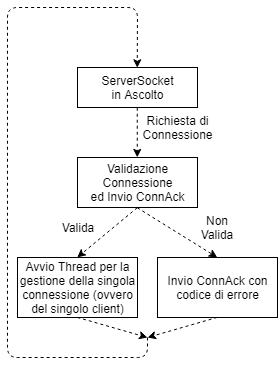
\includegraphics[scale=0.6]{immagini/serversocket.png}
\end{center}
Come si deduce dall'immagine ogni Client connesso con il Broker, viene gestito in un Thread separato. Quando la ServerSocket ci restituisce una Socket per comunicare con il Client appena connesso, il Broker attende l'arrivo del pacchetto Connect da parte del Client, controlla la validità del pacchetto, ed effetua l'autenticazione se necessaria, dopodichè risponde con una ConnAck che contiene l'esito della fase di connessione\\\\
Il thread che gestisce il client ``lato broker", si occupa di ricevere ed inviare messaggi, non appena avviato ricerca se è impostato il flag clean session a false, una sessione già esistente, altrimenti ne crea una nuova. Ogni sessione ha più code, o meglio code sincronizzate (siamo in ambiente concorrente), ognuna delle quali contiene differenti pacchetti, in accordo con la sezione relativa. In generale il comportamento di ogni thread, è rappresentato da un loop infinito, nel quale:
\begin{itemize}
	\item Vengono inviati tutti messaggi in attesa sulla coda di invio.
	\item Si leggono i messaggi in arrivo e li si processano a seconda della tipologia del messaggio.
	\item Si controlla il timer di keep alive, e se ha raggiunto il timeout, si chiude la connessione con il client (comportamento lato broker), o si invia una ping request (comportamento lato client.)
\end{itemize}

Ogni thread client, mette a disposizone un metodo per la pubblicazione di messaggi, che non fa altro che aggiungere il messaggio alla coda di invio, sarà il loop che invierà effetivamente il messsaggio. Quando si riceve un messaggio all'interno del loop, si ricostruisce il pacchetto, e si estrae la tipologia di esso, in base a ciò vengono intraprese differenti azioni, seguendo ciò che ho riportato nelle sezioni precedenti.\\\\
La gestione dei messaggi Retain, invece è stata implementata con una lista di messaggi pubblicati con flag retain, all'arrivo di un messaggio con il flag attivo, il messaggio viene aggiunto alla lista e quando un'nuovo client si connette, vengono automaticamente inviati i messaggi presenti nella lista, ma senza eliminarli, in quanto all'arrivo di un client, gli stessi messaggi devono essere pubblicati. Inoltre questa lista è indipendete dai client connessi, e ``sopravvive" fino a quando il Broker non viene terminato.

\subsection{Client}
Il client MQTT, possiede lo stesso loop di ricezione ed invio che ha il Broker, con l'unica differenza che quando il keep alive viene raggiunto, il client deve inviare un pacchetto di Ping Request al broker, e attendere una risposta (Ping Response), se questa non arriva entro un tempo limite pari anche'esso al keep alive, la connessione viene chiusa. La fase di connessione è stata implementata mediante l'utilizzo di Socket Java, che permettono l'invio successivamente del pacchetto di richiesta di connession MQTT (Connect), se il Broker risponde con un'ack di successo, entra in esecuzione il loop. La sessione per il client, contiene molte meno informazioni rispetto a quelle del broker, anche in questo caso per implementare la sessione sono state utilizzate code sincronizzate, per inserire e rimuovere i pacchetti ricevuti non confermati, e per quelli inviati non confermati. Rispetto al broker, a prescendire dal flag clean session, il client al momento della disconnessione elimina la sessione. Anche in questo caso il loop legge i pacchetti in arrivo, e in base alla tipologia di esso, intraprende differenti azioni. Riporto un piccolo esempio di come è possibile iscriversi a topic e pubblicare messaggi, aggiungo inoltre che è stata aggiunga un'interfaccia Java di callback per la ricezione di messaggi e per ottenere la conferma dei messaggi inviati in casi di Qos 1 e 2.
\begin{lstlisting}[style=JavaStyle]
// sottoscrizione
client.subscribe("/meteo/urbino",  Qos.QOS_2);
// pubblicazione
client.publish(new Message("/meteo/urbino", "soleggiato - 25.0", Qos.QOS_0, false));

// invocato alla ricezione di un messaggio
void onMessageArrived(Client client, Message message);

// invocato quando un messaggio con Qos > 0 viene consegnato.
void onDeliveryComplete(Client client, int messageId);

// invocata quando una sottoscrizione viene confermata.
void onSubscribeComplete(Client client, Subscribe subscribe);

\end{lstlisting}

\section{Conclusioni}
MQTT è effetivamente un protocollo ``semplice", che riesce a garantire con un'certo grado di sicurezza la consegna dei messaggi, si presta molto bene in applicazioni di IoT, dove dispositivi con poca potenza di calcolo e memoria limitata, possono communicare con il broker senza problemi, anche perchè il cliente deve fondamentalmente solo mantenere una connessione attiva. Stessa cosa per quanto riguarda l'occupazione di banda, con il giusto tempo di keep alive, i pacchetti scambiati sono essenzialmente pochi, e contengono solo informazioni realmente importanti. È facilmente implementabile in ogni linguaggi, non richiede strutture dati particolari.\\\\Aggiungo una considerazione sul lato sicurezza del protocollo, se supponiamo di avere un client che si sottoscrive ad un certo topic (client pippo), in fase di connessione esso si autentica mediante nome utente e password e con un determinato client id, ma imposta il flag di clean session a false, in modo tale che il broker mantenga in maniera permanente anche i topic a cui si è iscritto. Se ora siamo riusciti a determinare il client id, mediante un software di sniffing, possiamo collegarci con un altro client, con lo stesso id, e il broker ci darebbe accesso, e ci riconoscerebbe come client pippo, e riceveremmo tutti i messaggi destinati a pippo. Una possibile soluzione è quella di stabilire ID prefissati che il Broker conosce e da cui pretende l'autenticazione e ovviamente utilizzare un layer di trasporto sicuro, come TLS.

\end{document}